%% ------------------------------------------------------------------------- %%
\chapter{Desenvolvimento Experimental}
\label{cap:desenvolvimentos}

Este trabalho tem o objetivo de explorar possíveis soluções computacionais que sejam capazes de remover ou atenuar a contaminação telúrica de espectros astronômicos capturados a partir do solo. Para fazer isso é necessário um conhecimento aprofundado dos dados coletados, desde os procedimentos adotados na aquisição e redução de dados até interpretações astronômicas de características morfológicas desses sinais.

Neste capítulo são descritos os dados utilizados e os experimentos realizados durante o desenvolvimento do trabalho. Os experimentos foram úteis para permitir a visualização e compreensão dos espectros de ciência e telúrico, o teste do realinhamento de sinais como possível coadjuvante na remoção da contaminação telúrica, e o aprendizado de características fundamentais dos espectros na solução do problema da contaminação telúrica.  


\section{Formato de dados}

% o que é o formato fits
O formato de dados utilizado nos experimentos é o FITS ou \textit{Flexible Image Transfer System}~\citep{pence2010definition}. Este formato de arquivo digital facilita o armazenamento, processamento e transmissão de dados científicos e foi projetado para armazenar conjuntos de dados $n$-dimensionais que consistem em matrizes e tabelas. Este é o formato de dados mais utilizado na astronomia, possuindo recursos específicos para incluir informações de calibração fotométrica e espacial e outros metadados astronômicos relativos aos sinais armazenados.

% composição do arquivo fits
Um arquivo FITS é composto por segmentos chamados de HDU (\textit{Header-Data Units}) e ele deve necessariamente ter um \textit{Primary HDU}, que armazena os dados científicos principais. O \textit{PrimaryHDU} pode ser acompanhado de HDUs adicionais, categorizados entre extensões de imagens, extensões de tabelas ASCII e extensões de tabelas binárias \citep{nasa-fits}.

% header
O \textit{header} de um arquivo FITS contém uma lista de palavras-chave em letra maiúscula, associadas a um valor e possivelmente seguidas de um comentário. Estas palavras-chave representam elementos dos dados que são importantes, como a data de observação do arquivo, seu autor, seu histórico de processamento, seu telescópio de origem e também podem representar elementos relacionados à física da observação, como a massa de ar no momento e local de observação, temperatura ambiente, umidade e etc. A Fig. \ref{fig:fits-header} ilustra o \textit{header} típico de estrelas de ciência. 

\begin{figure}[htb]
\centering
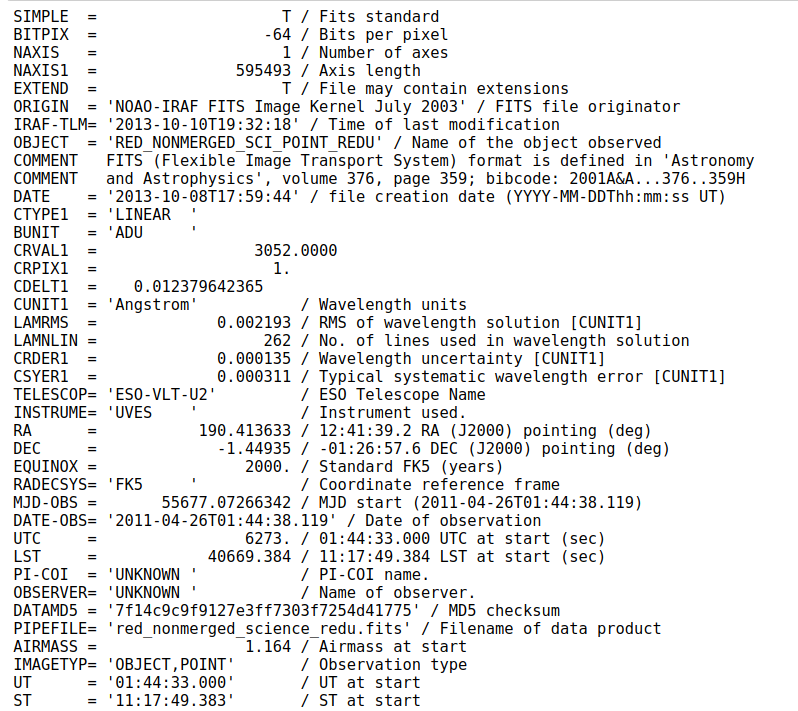
\includegraphics[width=10cm]{figuras/fits_header.png}
\caption{Trecho do cabeçalho do arquivo FITS da estrela HD110379}
\label{fig:fits-header}
\end{figure}

% data e tipos de dados
Dentro de uma HDU em um arquivo FITS, o componente em sequência ao \textit{header}, quando presente, possui um vetor que pode ter desde 1 até 999 dimensões. Esta seção representa o dado astronômico capturado, como os valores do fluxo de um espectro estelar ou uma imagem de um objeto celeste. Os dados podem ter um de 5 possíveis tipos de dados \citep{pence2010definition}:

\begin{enumerate}
    \item Inteiros de 8 bits
    \item Inteiros de 16 bits
    \item Inteiros de 32 bits
    \item Números reais de ponto flutuante de 32 bits
    \item Números reais de ponto flutuante de 64 bits
\end{enumerate}

\section{Ambiente e ferramentas}

%introduzir seção
A realização dos experimentos deste trabalho foi dependente de um conjunto de bibliotecas especializadas. Esta seção descreve as ferramentas utilizadas e detalhes da implementação dos experimentos.

% linguagem de programação: python
A linguagem de programação de escolha para a implementação dos experimentos foi o \textit{Python}, por esta permitir o uso de bibliotecas especializadas para o processamento de sinais e manipulação de dados astronômicos.

% jupyter notebooks
Os experimentos foram implementados em \textit{notebooks} do \textit{Jupyter}\footnote{\url{https://jupyter.org/}} \citep{Kluyver:2016aa}, um projeto de código-aberto com o objetivo de oferecer suporte à ciência de dados e computação científica interativa. Neste ambiente computacional é possível escrever código em células que podem ser executadas de forma independente. Esta interatividade faz com que os \textit{notebooks} sejam ambientes perfeitos para uma programação de natureza exploratória, já que é possível executar experimentos e apresentar resultados e gráficos entre várias células de código.

% pacotes python
Estabelecidos a linguagem e o ambiente dos experimentos, foram usadas diversas bibliotecas de \textit{Python} para ler, manipular e visualizar os dados estelares. Os pacotes utilizados foram: o \textit{NumPy}\footnote{\url{https://numpy.org/}} \citep{oliphant2006guide}, uma biblioteca fundamental de computação científica performática com suporte para vetores e matrizes grandes e multidimensionais, além de diversas funções matemáticas de alto nível; o \textit{Matplotlib}\footnote{\url{https://matplotlib.org/}} \citep{Hunter:2007}, uma biblioteca gráfica que permite a visualização de dados em diversos tipos de gráficos; e finalmente o \textit{Astropy}\footnote{\url{http://www.astropy.org}} \citep{astropy:2018}, uma biblioteca que é amplamente usado para processar computacionalmente diversos dados astronômicos e tem funcionalidades como leitura de arquivos FITS, conversões de unidades entre quantidades físicas e computações cosmológicas.

\section{Conjuntos de dados}

% datasets fornecidos: ardata, uves, molecfit e xsl (principal conjunto de dados)
Para o desenvolvimento dos experimentos destre trabalho, foram obtidos alguns conjuntos de dados estelares. Todos os arquivos destes conjuntos estão no formato FITS. Estes conjuntos de dados estelares englobam tanto observações reais de estrelas quando espectros telúricos sintéticos. A lista a seguir descreve estes conjuntos.

% lista dos dados 
\begin{itemize}
    \item UVES: dois pares de arquivos FITS contendo observações das estrelas HD110379 e HD110379 e seus respectivos referenciais telúricos. Estes dados foram capturados pelo espectrógrafo UVES \footnote{\url{https://www.eso.org/sci/facilities/paranal/instruments/uves.html}} \citep{2000SPIE.4008..534D}, instalado no \textit{Very Large Telescope Array} \footnote{\url{https://www.eso.org/public/brazil/teles-instr/paranal-observatory/vlt/?lang}}, no Cerro Paranal, Chile. Os dados foram obtidos como parte do \textit{proposal} de observação 087.B-0308(B), PI P. Coelho.
    \item FTS: uma tabela FITS contendo observações reais do Sol, da estrela Arcturus e um referencial telúrico para ambas \citep{arcturusflux:hinkle00}, observados pelo \textit{Fourier Transform Spectrometer} instalado no telescópio KPNO no National Optical Astronomy Observatory\footnote{\url{https://www.noao.edu/image_gallery/html/im0449.html}}.
    \item XSL: dados de observações do \textit{X-Shooter} \citep{Chen2014TheXS, unpublished-xshooter-data-release}, outro espectrógrafo que compõe o \textit{Very Large Telescope Array}. Mais detalhes sobre este conjunto de dados são explicados nesta seção (Anaïs Gonneau, comunicação privada).
    \item\texttt{Molecfit}: dados telúricos sintéticos gerados com a ferramenta \texttt{Molecfit} \citep{smette2015molecfit} 
\end{itemize}

% leitura dos dados
Antes de qualquer teste foi necessário um processo de ambientação e familiarização com os dados astronômicos. Para a leitura e manipulação de dados no formato FITS foi usada a biblioteca \textit{Astropy}.

% exemplos de estrelas mencionadas acima
A combinação dos dados com o ferramental adequado, possibilitou analisar e visualizar o espectro de diversas estrelas. Dois exemplos de estrelas de ciência e seus referenciais telúricos estão nas figuras~\ref{fig:two-stars-hd110379} e~\ref{fig:two-stars-sun}, e representam, respectivamente, a estrela HD110379 e o Sol. Além dos espectros completos, a figura~\ref{fig:two-stars-zoom-hd110379} ilustra dois painéis aumentados dos espectros observado e telúrico de HD110379, asim é possível ver as linhas espectrais com mais detalhes e compreender qual informação é perdida para a contaminação telúrica.

% observado e o telurico de cada um (ardata e uves)
\begin{figure}[!htb]
  \centering
  \subfloat[HD110379]{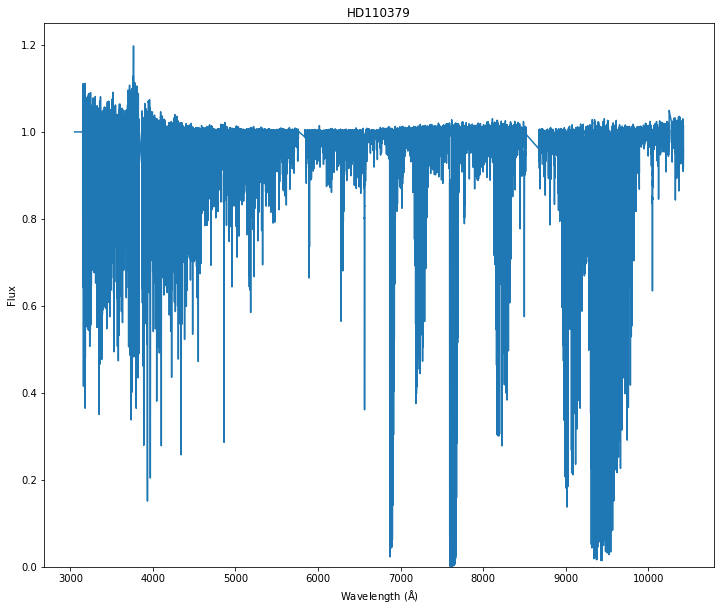
\includegraphics[width=0.5\textwidth]{figuras/hd110379_spectrum.png}\label{fig:hd110379}}
  \hfill
  \subfloat[Referência telúrica para HD110379]{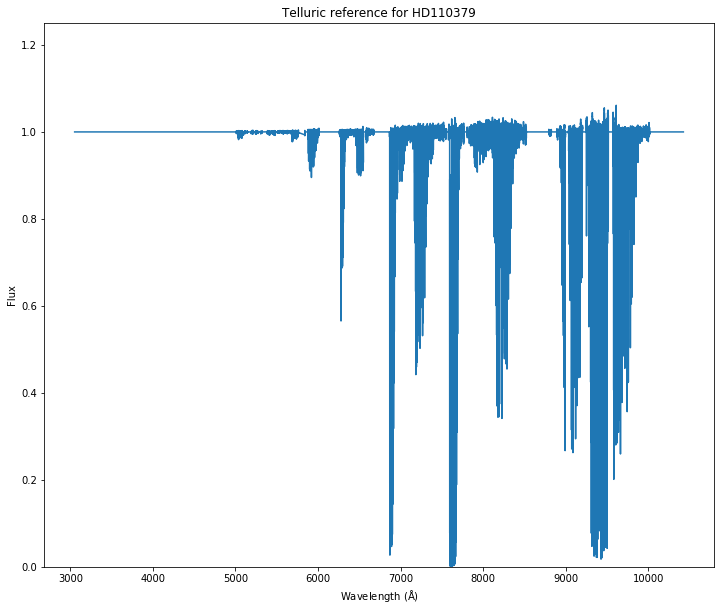
\includegraphics[width=0.5\textwidth]{figuras/hd110379_telluric.png}\label{fig:hd110379-tel}}
  \caption{Espectro observado com contaminação e espectro telúrico de HD110379}
  \label{fig:two-stars-hd110379}
\end{figure}

\begin{figure}[!htb]
  \centering
  \subfloat[HD110379]{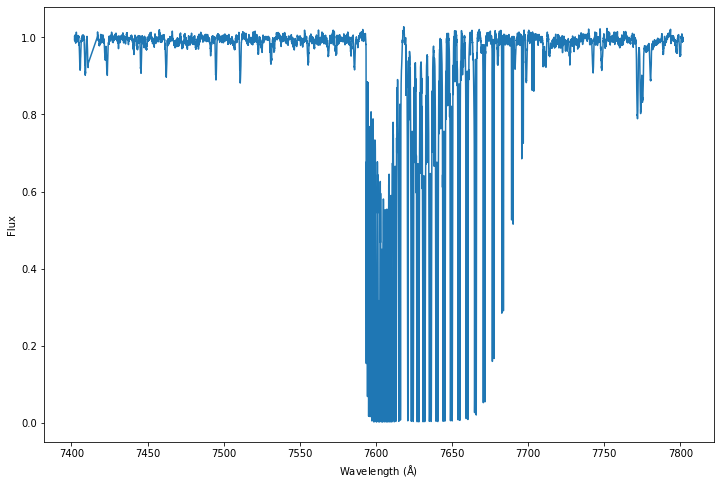
\includegraphics[width=0.5\textwidth]{figuras/hd110379_spectrum_zoom.png}\label{fig:hd110379-zoom}}
  \hfill
  \subfloat[Referência telúrica para HD110379]{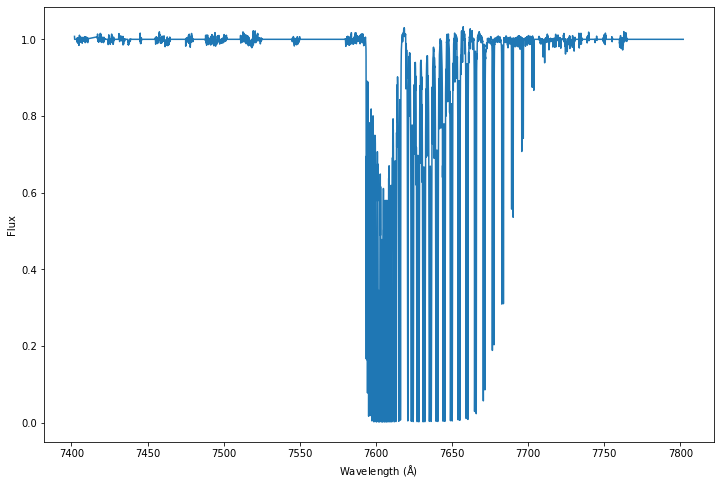
\includegraphics[width=0.5\textwidth]{figuras/hd110379_telluric_zoom.png}\label{fig:hd110379-tel-zoom}}
  \caption{Parte do espectro observado com contaminação e espectro telúrico de HD110379 no intervalo de comprimento de onda de 7400\mathrm{\AA} a 7800\mathrm{\AA}}
  \label{fig:two-stars-zoom-hd110379}
\end{figure}

\begin{figure}[htb]
  \centering
  \subfloat[Sol]{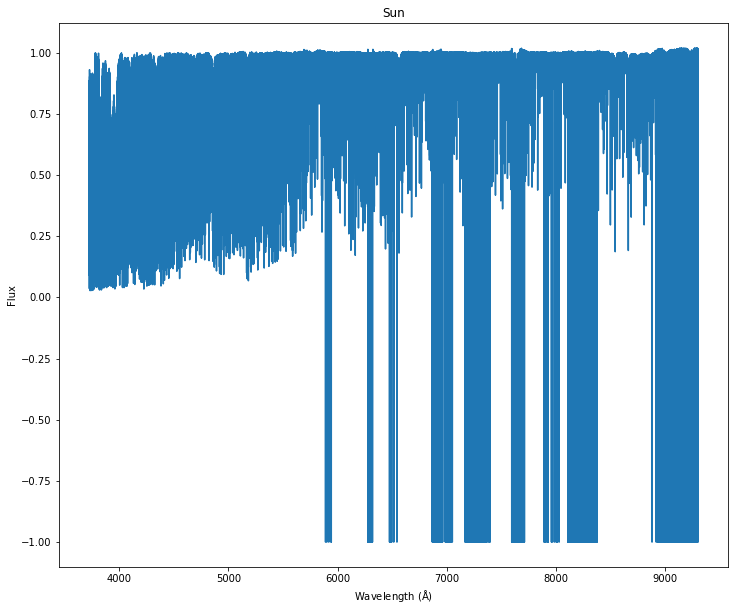
\includegraphics[width=0.5\textwidth]{figuras/sun_spectrum.png}\label{fig:sun}}
  \hfill
  \subfloat[Referência telúrica para o Sol]{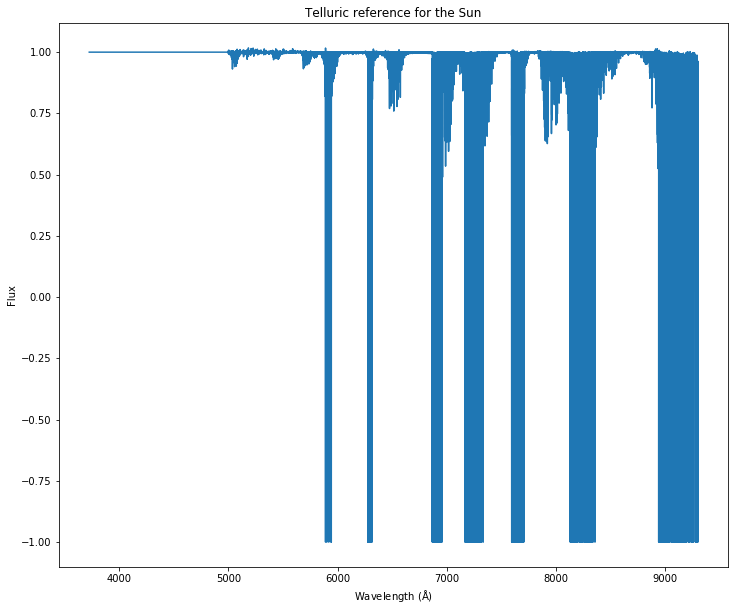
\includegraphics[width=0.5\textwidth]{figuras/sun_telluric.png}\label{fig:sun-tel}}
  \caption{Espectro observado com contaminação e espectro telúrico do Sol}
  \label{fig:two-stars-sun}
\end{figure}

% \mqz{Na figura 3.3 do Sol, o item (a) não é um espectro contaminado? O termo ``estrela de ciência'' é adequado para se referir a esse espectro?}

% seleção do xsl como dataset principal
Além das estrelas acima, como foi mencionado na seção~\ref{similarity-and-signal-alignment}, o principal conjunto de dados utilizado nos experimentos deste trabalho são estrelas do \textit{X-Shooter Spectral Library}. O diferencial deste conjunto de dados é que além das observações estelares e referenciais telúricos, foram fornecidos os espectros resultantes da correção telúrica. Desta maneira, foi possível estabelecer um \textit{ground truth} como base de comparação para os resultados dos experimentos. Neste conjunto de dados foram fornecidas quatro estrelas (X0319, X0386, X0538, X0771), com nove arquivos cada, distribuídos da seguinte maneira:

% mais detalhes sobre os dados do xsl (4 estrelas de ciencia, 4 teluricas sinteticas do molecfit e 4 corrigidas, dividas entre as regioes do espectro eletromagnetico infravermelho, visivel, ultravioleta)
\begin{itemize}
    \item *X\_N\_E.fits ou *X\_O\_E.fits: o espectro da estrela com contaminação telúrica, separado em 3 arquivos que cobrem intervalos de comprimento de ondas diferentes (X no nome do arquivo será U = ultravioleta, V = visível ou N = infravermelho);
    \item *TRA.fits: modelo \texttt{Molecfit} que representa o espectro telúrico correspondente ao dia da observação, também separado em 3 arquivos que cobrem comprimentos de ondas diferentes;
    \item *TAC.fits ou *TAC\_final.fits: espectros das estrelas corrigidos pelo modelo \texttt{Molecfit} e já considerando que as distorções observadas em comprimento de onda foram corrigidas, também separado em três arquivos.
\end{itemize}

% plotar os espectros do xsl nas unidades que vieram e falar das diferenças entre os obs e teluricos (escalase formatos) e diferenca com figuras anteriores
\begin{figure}[htb]
  \centering
  \subfloat[X0319 observado]{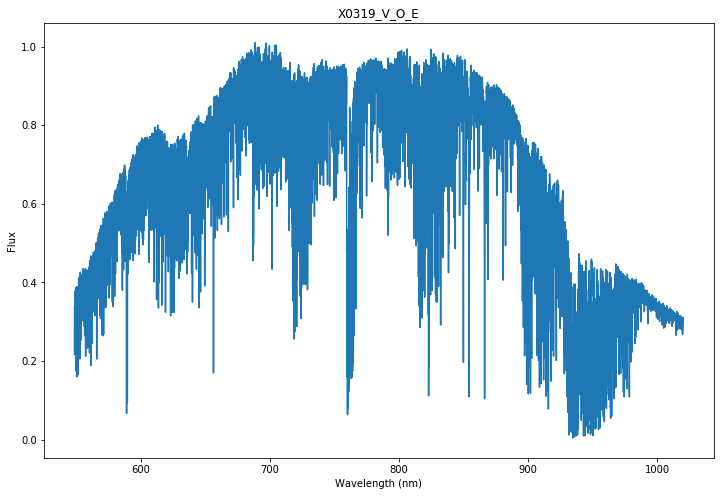
\includegraphics[width=0.5\textwidth]{figuras/x0319_v_o_e.png}\label{fig:x0319-v-o-e}}
  \hfill
  \subfloat[Referência telúrica para X0319]{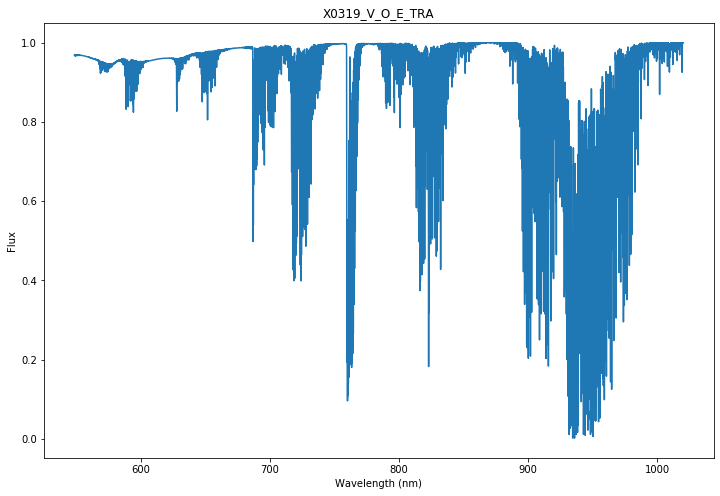
\includegraphics[width=0.5\textwidth]{figuras/x0319_v_o_e_tra.png}\label{fig:x0319-v-o-e-tra}}
  \caption{Espectro observado com contaminação e espectro telúrico de X0319 na região visível de comprimento de onda}
  \label{fig:x0319-visible}
\end{figure}


\begin{figure}[htb]
  \centering
  \subfloat[X0386 observado]{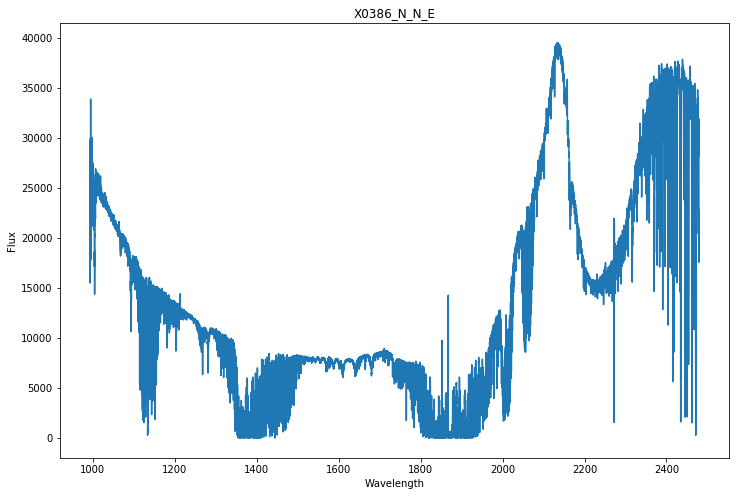
\includegraphics[width=0.5\textwidth]{figuras/x0386_n_n_e.png}\label{fig:x0386-n-n-e}}
  \hfill
  \subfloat[Referência telúrica para X0386]{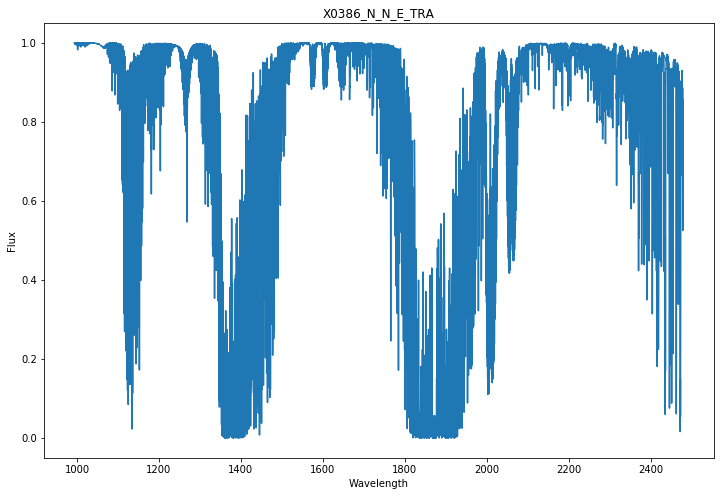
\includegraphics[width=0.5\textwidth]{figuras/x0386_n_n_e_tra.png}\label{fig:x0386-n-n-e-tra}}
  \caption{Espectro observado com contaminação e espectro telúrico de X0386 na região infravermelho de comprimento de onda}
  \label{fig:x0386-infrared}
\end{figure}


\begin{figure}[htb]
  \centering
  \subfloat[X0538 observado]{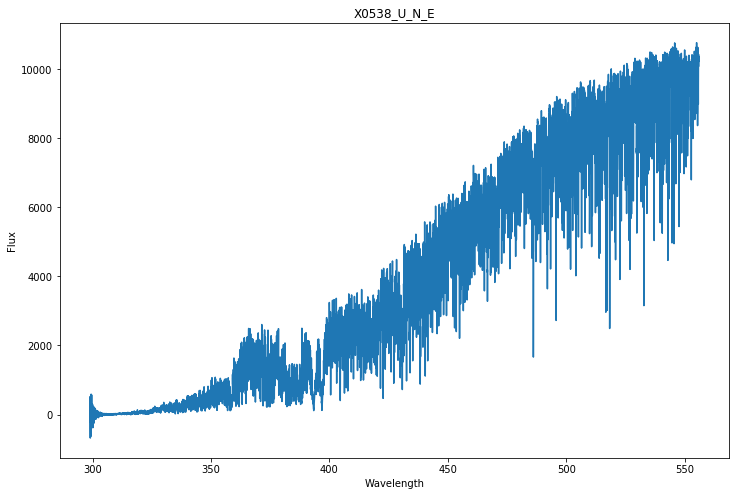
\includegraphics[width=0.5\textwidth]{figuras/x0538_u_n_e.png}\label{fig:x0538-u-n-e}}
  \hfill
  \subfloat[Referência telúrica para X0538]{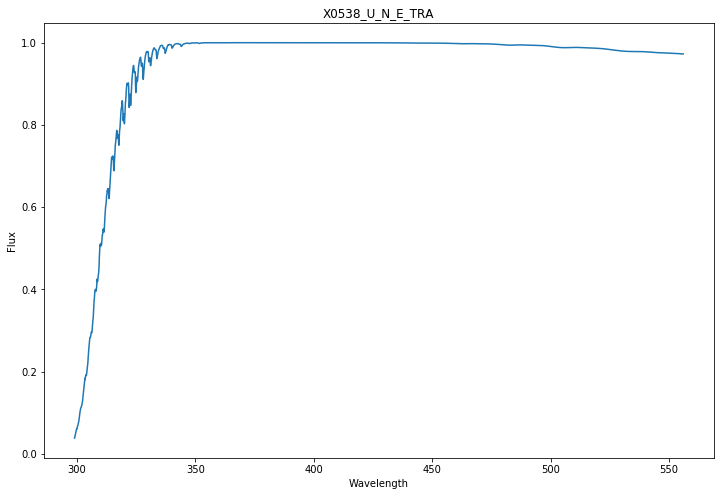
\includegraphics[width=0.5\textwidth]{figuras/x0538_u_n_e_tra.png}\label{fig:x0538-u-n-e-tra}}
  \caption{Espectro observado com contaminação e espectro telúrico de X0538 na região ultravioleta de comprimento de onda}
  \label{fig:x0538-ultraviolet}
\end{figure}

As figuras~\ref{fig:x0319-visible},~\ref{fig:x0386-infrared} e~\ref{fig:x0538-ultraviolet} ilustram exemplos de alguns espectros do conjunto de dados do \textit{X-Shooter}, tanto de diferentes estrelas quanto de diferentes regiões de comprimentos de onda. 

% falar sobre diferença no eixo y 
Uma das diferenças entre o espectro observado e o telúrico de uma mesma estrela é a diferença de ordem de magnitude da escala do eixo y dos gráficos. Como foi mencionado na seção~\ref{data-reduction}, os espectros observados possuem uma unidade física ao final do processo de redução de dados. No caso das observações do conjunto de dados do \textit{X-Shooter} utilizadas nesse trabalho, os espectros não passaram pelo processo de redução de dados por completo. Nesse caso o eixo y não possui o mesmo significado físico de intensidade por unidade de área, tempo e comprimento de onda, mas é uma quantidade adimensional relacionada ao número de fótons detectado pelo CCD.

% tentar introduzir o significado do eixo e explicação da adimensionalidade do fluxo antes do final da redução de dados
Como o fluxo é capturado pelo CCD através da corrente elétrica produzida por uma certa contagem de fótons, o processo de conversão entre a tensão produzida no instrumento e finalmente uma unidade fisicamente interpretável é extremamente sofisticado em termos de \textit{hardware} e não será abordado neste trabalho. Para os experimentos realizados neste capítulo é importante notar que o eixo y é relacionado tanto ao fluxo da estrela quanto à assinatura instrumental do espectrógrafo. 

% espectro do molecfit e normalização pro intervalo [0,1]
Já nos espectros telúricos sintéticos do \texttt{Molecfit}, o eixo y do gráfico é normalizado para o intervalo $[0, 1]$ e representa um mapa de transmitância da atmosfera, ou seja, uma série de fatores de absorção que quando interagem com o sinal estelar capturam parte da sua emissão. Para facilitar o restante dos experimentos, as observações do \textit{X-Shooter} também tiveram seus intervalos normalizados de forma a simplificar a manipulação dos dados.

\section{Divisão do sinal estelar pelo telúrico}

% introdução à motivação por tras deste experimento
% queremos validar com os dados em maos que a divisão de fato não é a melhor solução para o problema e entender qual seria a consequencia dela nestas observações
Após o processo de exploração e familiarização com os dados astronômicos fornecidos, o primeiro experimento idealizado neste trabalho foi a divisão dos espectros estelares observados pelas suas respectivas referências telúricas, a fim de evidenciar as limitações desse processo.
% recapitular pq podemos dividir os espectros
Como mencionado na seção~\ref{telluric-contamination}, por causa da natureza multiplicativa do modelo físico da transmissão da radiação estelar através da atmosfera, a correção telúrica corresponderia de fato à divisão simples entre os espectros de ciência e telúrico. A motivação por trás deste experimento é observar que na prática esta solução não é ideal e cria artefatos no espectro estelar. 

Algumas explicações do porquê o método da correção telúrica pela divisão simples de espectros não funciona como proposto no modelo teórico provêm das distorções do sinal que possuem origem instrumental. Alguns exemplos de distorções esperadas pelos astrônomos em suas observações são o alargamento das linhas espectrais, desconsiderando o alargamento Doppler \citep{LEVENHAGEN2008}, e a criação de deslocamentos no domínio de comprimento de onda provenientes de artefatos de \textit{hardware} \citep[e.g.][]{wavelength-shifts}.
% mostrar resultados de alguns conjuntos de dados que ilustrem bem a criação de artefatos 
A primeira divisão realizada foi do conjunto de dados do espectrógrafo UVES, na estrela HD110379. 

\begin{figure}[htb]
  \centering
  \subfloat[HD110379]{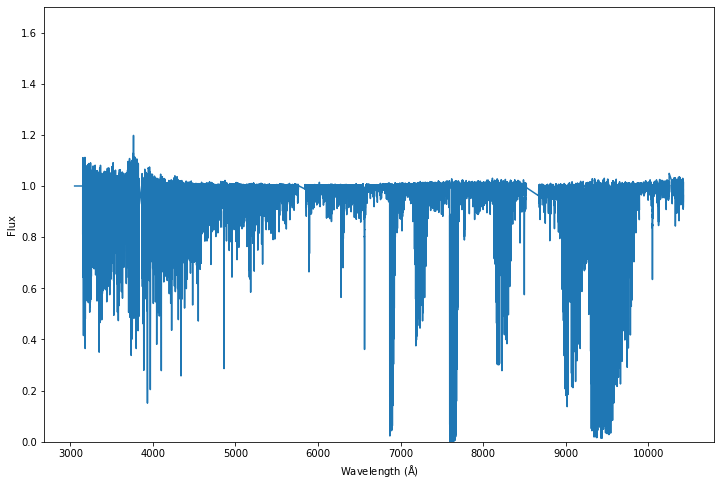
\includegraphics[width=0.5\textwidth]{figuras/hd110379_spectrum_scaled.png}\label{fig:hd110379-spectrum-scaled}}
  \hfill
  \subfloat[Resultado da correção telúrica HD110379]{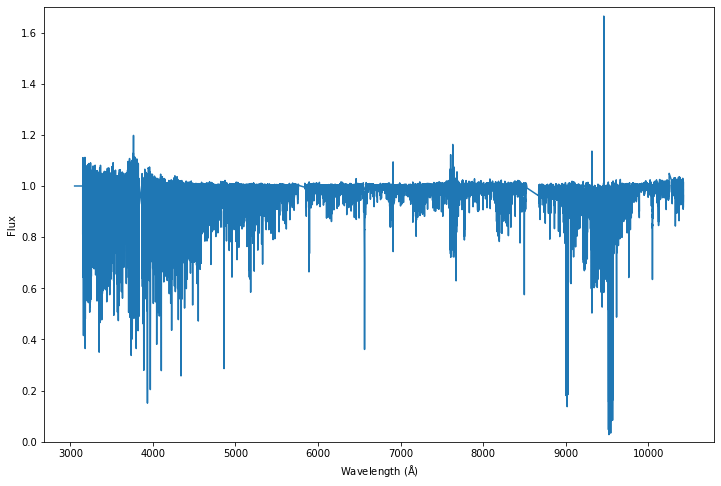
\includegraphics[width=0.5\textwidth]{figuras/hd110379_divided.png}\label{fig:hd110379-divided}}
  \caption{Espectros de ciência e dividido de HD110379 pelo seu referencial telúrico}
  \label{fig:hd110379-division}
\end{figure}

Na figura~\ref{fig:hd110379-division}, temos o espectro de ciência original da estrela HD110379 e o resultado da correção telúrica que é a divisão simples entre os espectros. Ambos tiveram seus eixos y redimensionados de modo a facilitar a inspeção visual dos resultados.  A correção telúrica neste caso de fato diminui algumas das linhas de absorção do espectro, principalmente na região dos 6500$\mathrm{\AA}$ aos 8500$\mathrm{\AA}$ de comprimento de onda. Porém, é visivelmente perceptível que ela também cria artefatos como picos no espectro resultante, sendo alguns menores e outros maiores quando comparados ao intervalo [0, 1] do fluxo estelar.

\begin{figure}[htb]
  \centering
  \subfloat[X0319]{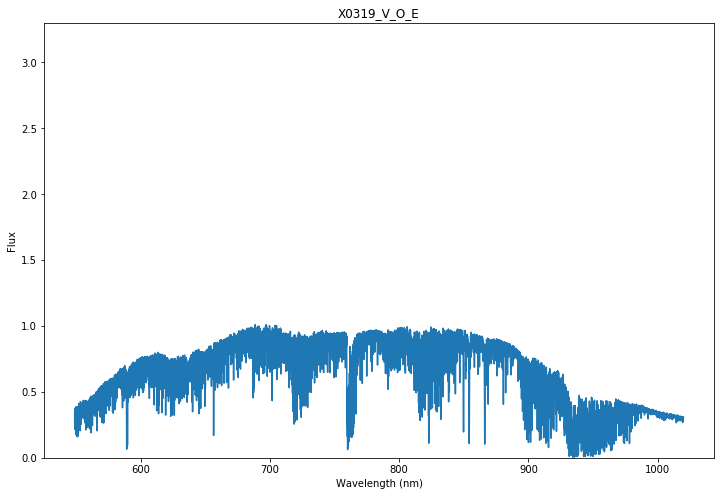
\includegraphics[width=0.5\textwidth]{figuras/x0319_v_o_e_scaled.png}\label{fig:x0319-spectrum-scaled}}
  \hfill
  \subfloat[Resultado da correção telúrica X0319]{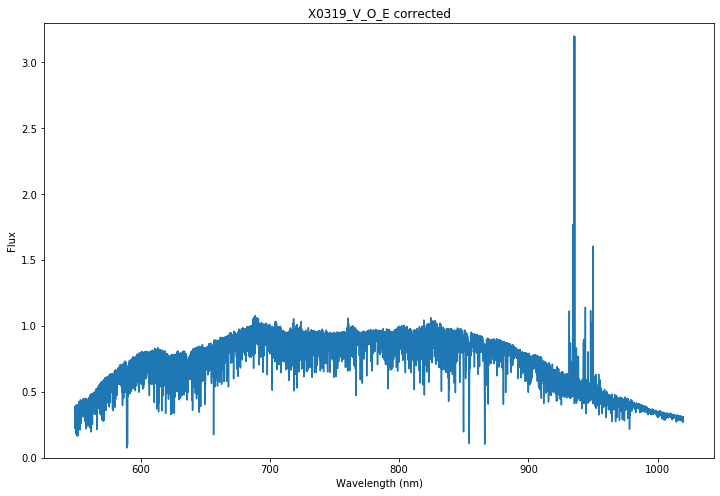
\includegraphics[width=0.5\textwidth]{figuras/x0319_v_o_e_divided.png}\label{fig:x0319-divided}}
  \caption{Espectros de ciência e dividido de X0319 pelo seu referencial telúrico}
  \label{fig:x0319-division}
\end{figure}

A figura~\ref{fig:x0319-division} mostra mais um exemplo de correção telúrica feita nos dados fornecidos, desta vez na estrela X0319 do espectrógrafo \textit{X-Shooter}. Novamente, os eixos dos gráficos dos espectros foram redimensionados, de modo a facilitar a visualização dos efeitos da divisão do observado pelo telúrico. Neste caso, é possível observar tanto a diminuição das linhas de absorção ao longo do espectro, quanto a criação de picos no mesmo, principalmente na região entre 900nm e 1000nm, na qual o pico resultante tem uma escala aproximadamente três vezes maior que a do espectro original.

% picos de sinal podem ter sido causados pos shifts em regiões do espectro
Os artefatos criados pelas correções telúricas das figuras acima não deveriam existir na situação ideal do problema, onde, elemento a elemento, o fluxo do espectro de ciência deveria ser maior ou igual ao fluxo após a absorção atmosférica representada pelo espectro telúrico. Isto indica a presença de um dos efeitos esperados deste tipo de operação: o desalinhamento entre o espectro estelar e o telúrico. Os resultados das correções telúricas e os seus efeitos resultantes fazem sentido, principalmente no caso da estrela do \textit{X-Shooter}, onde pesquisadores observaram estes mesmos problemas \citep{unpublished-xshooter-data-release, wavelength-shifts}

% passar pra dtw e a tentativa de resolver os desalinhamentos
Os resultados das divisões nesta seção ilustram as dificuldades conhecidas no processo atual de correção telúrica e deixam explícita a necessidade propor soluções alternativas que melhorariam a qualidade dos dados observados.

\section{DTW no sinal estelar}

% introdução da seção
Os resultados do experimento de correção telúrica através da divisão de um espectro estelar pelo seu referencial telúrico esclarecem a necessidade de considerar melhorias ao processo atual. Como foi visto, um dos problemas nos dados é a falta de alinhamento entre os sinais, e a consequente criação de artefatos e distorções nos espectros corrigidos. O experimento desta seção propõe uma solução alternativa a uma das dificuldades conhecidas das observações: o desalinhamento dos espectros.

% decisão de usar dtw
Como foi explicado na seção~\ref{similarity-and-signal-alignment}, podemos usar o algoritmo \textit{Dynamic Time Warping}, representado pelos algoritmos~\ref{dtw-matrix} e~\ref{dtw-path}, para encontrar o alinhamento ótimo entre dois sinais, e o algoritmo~\ref{dtw-realignment} para realinhar os sinais em relação ao resultado do DTW. Assim, seria possível realinhar o espectro da observação estelar com o espectro telúrico para resultar em uma divisão de maior qualidade e menor perda de informação e criação de artefatos. 

% dados utilizados no experimento e versão do DTW
Para este experimento o conjunto de dados utilizado foi o XSL e a implementação do DTW foi a \textit{FastDTW}, de modo a permitir a aplicação do algoritmo nos espectros completos (ou seja, em todas as faixas de comprimentos de onda).

% primeiro experimento
O primeiro exemplo da aplicação do DTW nos dados da XSL considera todo o intervalo visível de comprimento de onda da estrela X0319, cujos espectros são ilustrados na figura~\ref{fig:x0319-visible}. O algoritmo foi aplicado nos espectros estelar e telúrico, e o caminho gerado pelo DTW está na figura~\ref{fig:x0319-warp-path}.

\begin{figure}[htb]
\centering
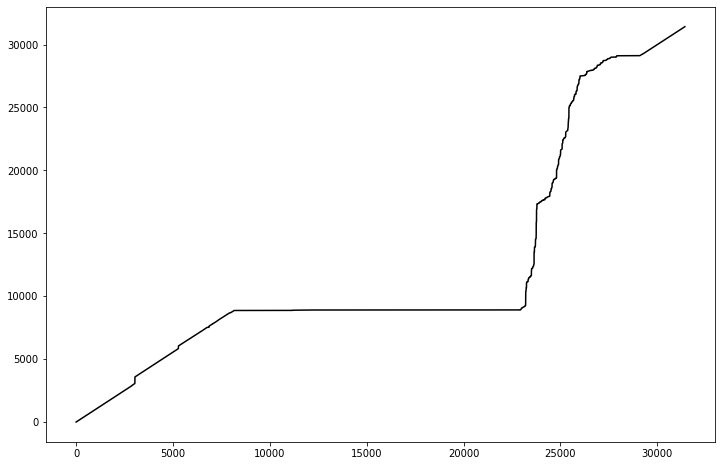
\includegraphics[width=10cm]{figuras/x0319_warp_path.png}
\caption{Caminho do DTW para o espectro estelar e telúrico de X0319}
\label{fig:x0319-warp-path}
\end{figure}

O caminho resultante do algoritmo já indica uma série de regiões problemáticas dos espectros que não puderam ser alinhadas de maneira razoável. Idealmente o caminho deveria se distanciar pouco da diagonal secundária da matriz de similaridade, mas neste caso são claras as regiões onde as sequências simplesmente não são similares, como a linha horizontal que ocupa a maioria do caminho, seguida de um trecho quase vertical.

O espectro telúrico original do \texttt{Molecfit} e o realinhado em relação à observação estelar que foi reconstruído a partir do caminho do DTW estão apresentados na figura~\ref{fig:x0319-realigned-telluric}.

\begin{figure}[htb]
  \centering
  \subfloat[Modelo telúrico do \texttt{Molecfit} de X0319]{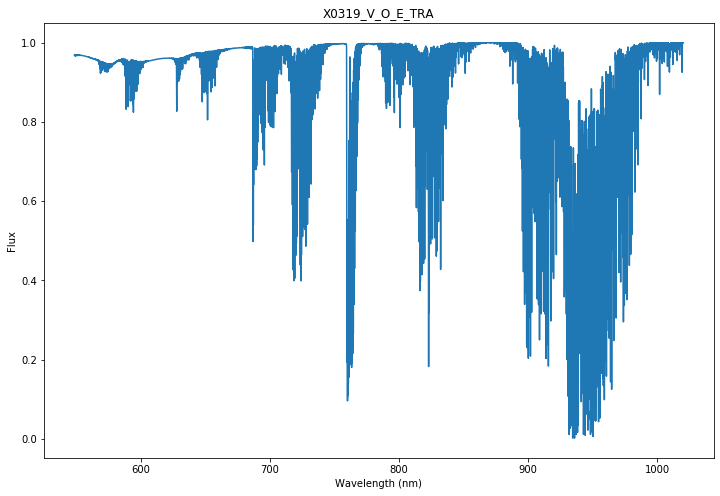
\includegraphics[width=0.5\textwidth]{figuras/x0319_v_o_e_tra.png}}
  \hfill
  \subfloat[Espectro telúrico de X0319 realinhado]{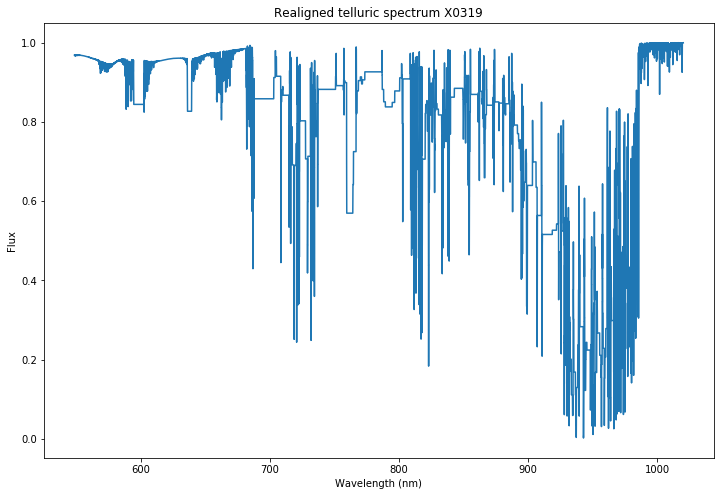
\includegraphics[width=0.5\textwidth]{figuras/x0319_v_o_e_aligned.png}}
  \caption{Espectro telúrico de X0319 e espectro telúrico realinhado a partir do caminho do DTW}
  \label{fig:x0319-realigned-telluric}
\end{figure}

% resultado do espectro telurico realinhado
É possível ver que, por mais que o espectro telúrico realinhado da estrela X0319 tenha o formato geral do modelo do \texttt{Molecfit}, ele possui uma forte distorção em relação às linhas espectrais originais e exibe a formação de ângulos retos que não são característicos deste tipo de dado.

% mais um exemplo em outra estrela no espectro completo
O próximo teste também foi feito em uma estrela do XSL, a estrela X0386, no intervalo visível de comprimento de onda do espectro. A escolha desta região espectral se deve ao fato de que a contaminação telúrica está presente, porém é menos intensa e de mais difícil correção do que na região de comprimento de onda infravermelho. Quanto à região ultravioleta, esta parece ser menos sensível aos efeitos da atmosfera terrestre, como pode ser visualizado na figura \ref{fig:molectfit-telluric-reference}.

% espectro observado, porque não foi mostrado antes
A figura~\ref{fig:x0386-v-n-e} a seguir ilustra a observação estelar de X0386, para que se possa perceber o formato do espectro contaminado.

\begin{figure}[htb]
\centering
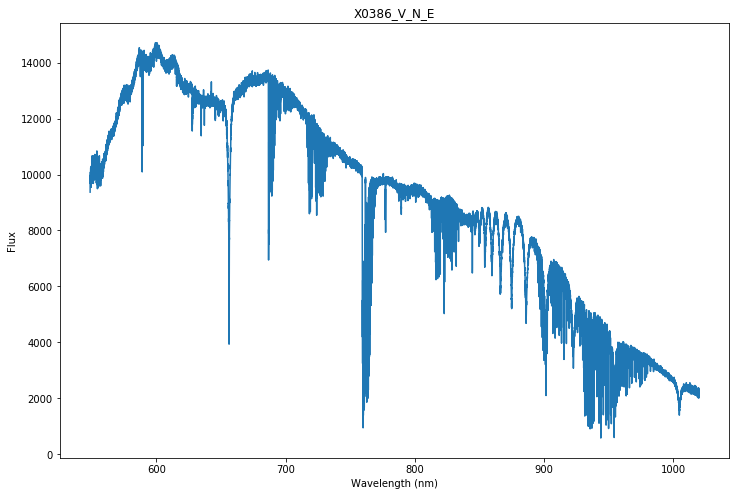
\includegraphics[width=10cm]{figuras/x0386_v_n_e_spectrum.png}
\caption{Espectro observado com contaminação telúrica de X0386}
\label{fig:x0386-v-n-e}
\end{figure}

% comentarios do caminho do DTW
Nesta observação e no seu referencial telúrico foi aplicado o DTW, e a figura~\ref{fig:x0386-warp-path} contém o caminho resultante do algoritmo. Neste caso também é possível observar que o caminho apresenta uma grande distorção em relação à diagonal ideal, o que significa que o sinal estelar e telúrico não possuem um alinhamento razoável que permitiria a divisão simples dos espectros.

\begin{figure}[htb]
\centering
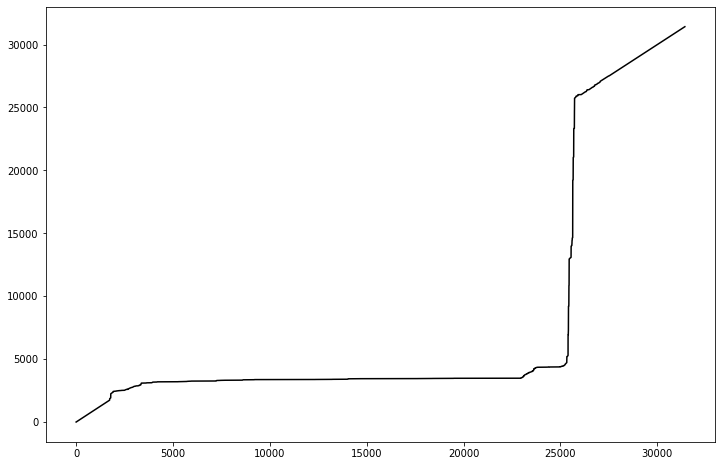
\includegraphics[width=10cm]{figuras/x0386_warp_path.png}
\caption{Caminho do DTW para o espectro estelar e telúrico de X0386}
\label{fig:x0386-warp-path}
\end{figure}

% resultados do algoritmo no realinhamento 
Os efeitos da distorção causada pelo realinhamento de espectro telúrico usando o caminho resultante do DTW podem ser vistos na figura~\ref{fig:x0386-realigned-telluric}. O espectro telúrico realinhado sofre uma grande perda de informação nas suas linhas espectrais e é possível ver que ele se assemelha ao modelo original apenas no intervalo entre 900nm e 1000nm, a mesma região do caminho do DTW que se aproxima da diagonal secundária da matriz de similaridade.

% espectro telurico e realinhado de x0386
\begin{figure}[H]
  \centering
  \subfloat[Modelo telúrico do \texttt{Molecfit} de X0386]{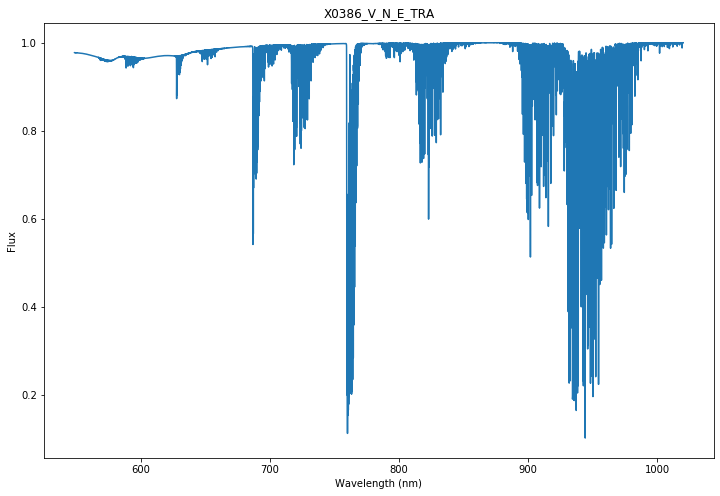
\includegraphics[width=0.5\textwidth]{figuras/x0386_v_n_e_tra.png}}
  \hfill
  \subfloat[Espectro telúrico de X0386 realinhado]{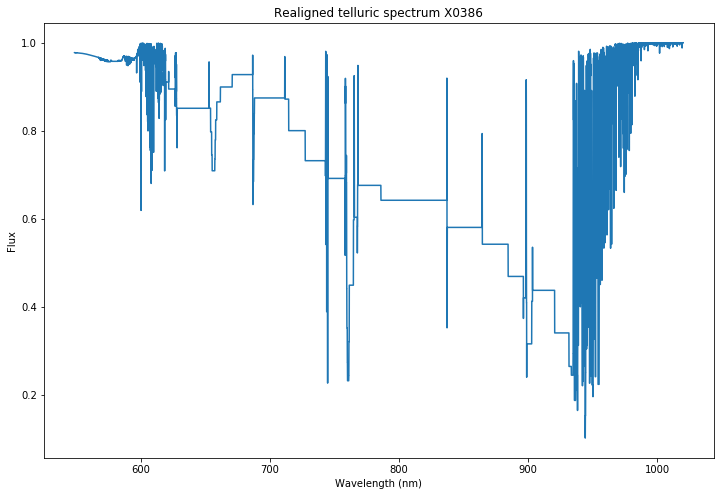
\includegraphics[width=0.5\textwidth]{figuras/x0386_v_n_e_aligned.png}}
  \caption{Espectro telúrico de X0386 e espectro telúrico realinhado a partir do caminho do DTW}
  \label{fig:x0386-realigned-telluric}
\end{figure}


% mais um exemplo com zoom no espectro para mostrar as linhas e os efeitos no nível micro
Uma hipótese para explicar o baixo desempenho da aplicação do DTW nos espectros completos seriam as grandes diferenças de perfil global que se observam entre os espectros de ciência e os espectros telúricos: a intuição que levou à seleção do DTW como ferramenta de alinhamento entre esses espectros diferentes correspondia à similaridade observável nesses espectros entre as linhas de absorção correspondentes a elementos químicos específicos. Assim, um próximo passo natural correspondia a testar o algoritmo de realinhamento em regiões menores do espectro.

Para verificar essa nova hipótese, foi aplicado o DTW no espectro da estrela X0319, no intervalo de comprimento de onda entre 834nm e 841nm. As figuras~\ref{fig:x0319-warp-path-zoom} e~\ref{fig:x0319-realigned-telluric-zoom} mostram o caminho resultante na matriz de similaridade e o espectro telúrico original e realinhado. 
\begin{figure}[htb]
\centering
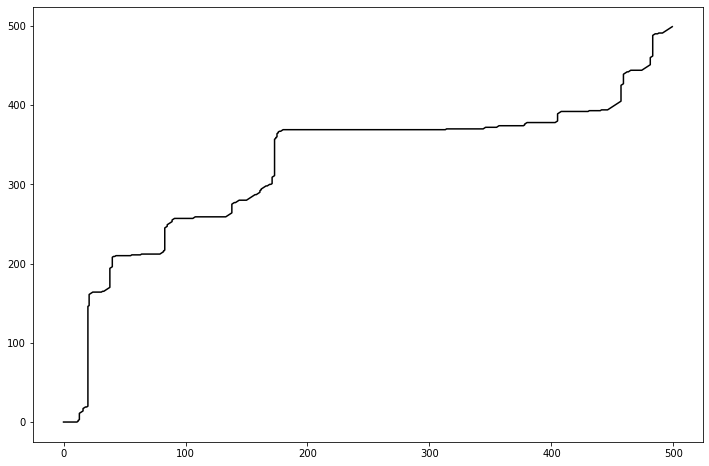
\includegraphics[width=10cm]{figuras/x0319_warp_path_zoom.png}
\caption{Caminho do DTW para o espectro estelar e telúrico de X0319 no intervalo de 834nm a 841nm}
\label{fig:x0319-warp-path-zoom}
\end{figure}

\begin{figure}[H]
  \centering
  \subfloat[Modelo telúrico do \texttt{Molecfit} de X0319]{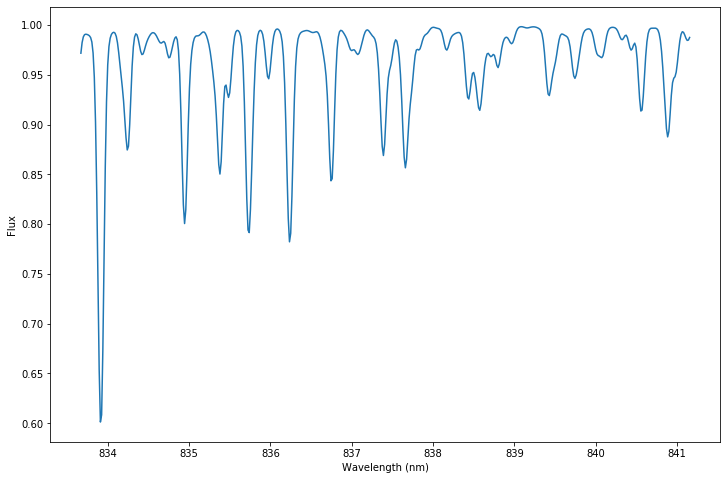
\includegraphics[width=0.5\textwidth]{figuras/x0319_v_o_e_tra_zoom.png}}
  \hfill
  \subfloat[Espectro telúrico de X0319 realinhado]{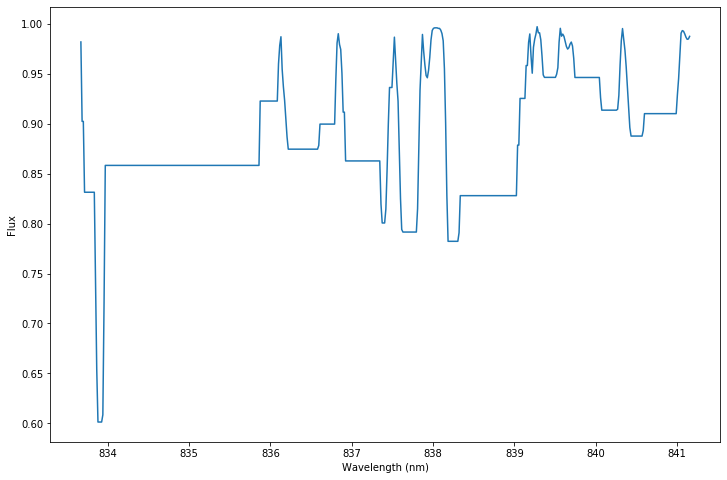
\includegraphics[width=0.5\textwidth]{figuras/x0319_v_o_e_aligned_zoom.png}}
  \caption{Espectro telúrico de X0319 e espectro telúrico realinhado a partir do caminho do DTW no intervalo de 834nm a 841nm}
  \label{fig:x0319-realigned-telluric-zoom}
\end{figure}

Neste experimento são observados os mesmos problemas dos experimentos anteriores em menor escala. Em um intervalo de comprimento de onda que abrange 9nm de espectro estelar ocorrem os mesmos deslocamentos horizontais e verticais no caminho da matriz de similaridades, e no espectro telúrico realinhado também ocorre a formação de ângulos retos nas linhas de absorção.

% conclusoes deste experimento
A aplicação do \textit{Dynamic Time Warping} entre o sinal estelar e o modelo telúrico não se mostrou adequado para alinhar as linhas de absorção correspondentes nesses espectros permitindo assim a correção da distorção telúrica. O algoritmo, que se baseia na premissa de forte similaridade entre os conteúdos a serem alinhados, não produz alinhamentos razoáveis quando aplicado em sinais que não representam a mesma informação, embora compartilhem regiões com linhas de absorção de origens equivalentes. O DTW ainda poderia funcionar, hipoteticamente, em um caso onde fosse possível isolar setores muito pequenos, com linhas de absorção similares e claramente separadas.


\section{DTW no sinal atmosférico}

% introdução do experimento
Os experimentos de uso do \textit{Dynamic Time Warping} como ferramenta de realinhamento entre o sinal estelar e o referencial telúrico contribuíram para uma maior familiarização em relação aos dados usados neste trabalho e também introduziram questionamentos sobre o sinal atmosférico obtido do \texttt{Molecfit}.

% como os pesquisadores do xsl resolveram o problema dos desalinhamentos
Os pesquisadores do XSL, ao identificarem os desalinhamentos nos espectros resolveram o problema dividindo o sinal em sub-espectros, e para cada um destes utilizaram o \texttt{Molecfit} para recomputar o modelo telúrico neste intervalo de comprimento de onda. Esta solução tem o objetivo de empiricamente obter o \textit{shift} único de cada sub-espectro. A partir deste procedimento foi realizada a correção telúrica nos espectros do XSL, como é descrito no artigo de \citet{unpublished-xshooter-data-release}.

% como resgatar atm' e por que
Com os dados fornecidos dos espectros estelares corrigidos que são considerados como o \textit{ground-truth} neste trabalho, é possível resgatar o espectro telúrico realinhado a partir da divisão do espectro estelar observado pelo espectro estelar corrigido. Desta forma, se temos os vetores $o$ e $c$ que representam a observação contaminada e o espectro final corrigido, teríamos o espectro real de transmitância da atmosfera dado por

\begin{equation*}
    a' = o \oslash c \qquad \left(\mbox{ou equivalentemente:} \qquad a'_{i} = o_i / c_i,\ \forall i\right),
\end{equation*}

\noindent onde $a'$ representa o espectro telúrico com correção dos desalinhamentos observados ($\oslash$ denota a divisão de Hadamard).

% desalinhamento entre os espectros atmosfericos gt e molecfit
O estudo do sinal atmosférico corrigido em relação ao modelo telúrico do \texttt{Molecfit} permite obter mais informações sobre os dados e entender o quão grande é o desalinhamento entre estes espectros. Os experimentos desta seção se propõem a resgatar o sinal atmosférico correspondente ao \textit{ground-truth} e compará-lo com o sinal atmosférico obtido com o conjunto de dados do XSL.

% estrelas usadas
As estrelas utilizadas para este experimento são a X0319 e a X0386 do \textit{X-Shooter Spectral Library}, na região visível de comprimento de onda. As figuras~\ref{fig:x0319-gt-telluric} e~\ref{fig:x0386-gt-telluric} mostram os modelos telúricos dados e os seus respectivos espectros telúricos realinhados a partir da divisão entre a observação estelar com contaminação telúrica e o espectro corrigido \citep{unpublished-xshooter-data-release}.

% mostrar os gts recuperados para duas estrelas
\begin{figure}[htb]
  \centering
  \subfloat[Modelo telúrico do \texttt{Molecfit} de X0319]{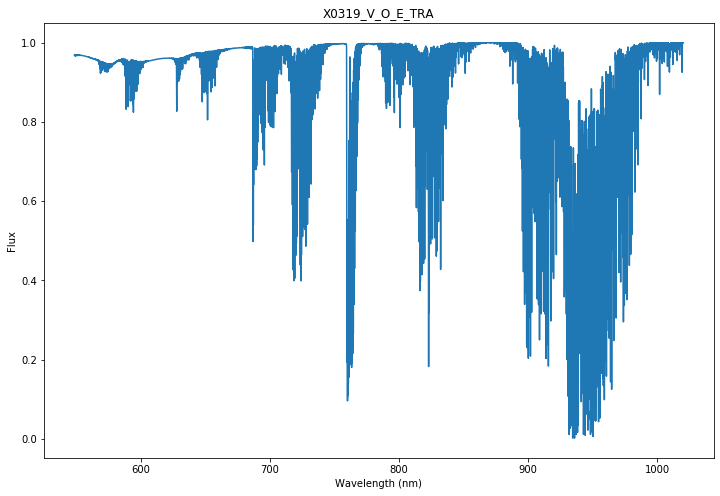
\includegraphics[width=0.5\textwidth]{figuras/x0319_v_o_e_tra.png}}
  \hfill
  \subfloat[Espectro telúrico de X0319 realinhado]{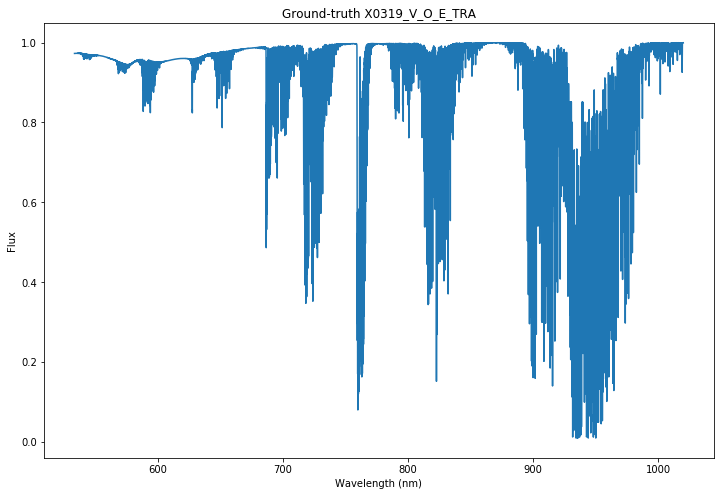
\includegraphics[width=0.5\textwidth]{figuras/x0319_v_o_e_tra_gt.png}}
  \caption{Espectro telúrico dado e espectro telúrico corrigido de shifts de X0319}
  \label{fig:x0319-gt-telluric}
\end{figure}

\begin{figure}[htb]
  \centering
  \subfloat[Modelo telúrico do \texttt{Molecfit} de X0386]{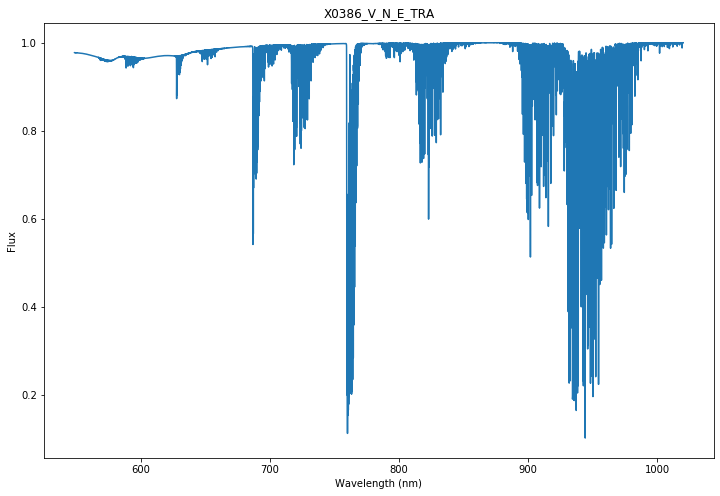
\includegraphics[width=0.5\textwidth]{figuras/x0386_v_n_e_tra.png}}
  \hfill
  \subfloat[Espectro telúrico de X0386 realinhado]{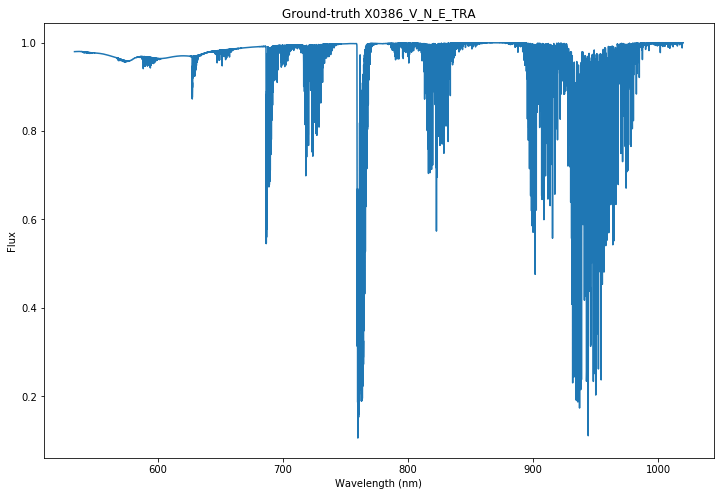
\includegraphics[width=0.5\textwidth]{figuras/x0386_v_n_e_tra_gt.png}}
  \caption{Espectro telúrico dado e espectro telúrico corrigido de shifts de X0386}
  \label{fig:x0386-gt-telluric}
\end{figure}

% características dos sinais gt
Por inspeção visual, é possível observar que os espectros corrigidos de desalinhamentos não possuem distorções perceptíveis em relação aos seus correspondentes modelos do \texttt{Molecfit}. Isto indica que se existem desalinhamentos entre estes sinais, estes devem ser pequenos. 

% dtw nestes sinais: deveria funcionar bem melhor agora que os espectros representam a mesma informação 
A presença de pequenos desalinhamentos entre os sinais sugere que estes dados seriam adequados à aplicação do algoritmo do \textit{Dynamic Time Warping}. Desta forma seria possível observar regiões com maior desalinhamento, e portanto, quais regiões do espectro tiveram correções de \textit{shifts} feitas pelo grupo de pesquisadores que lidaram com estes espectros.

% mostrar resultados do DTW nas duas estrelas e com zoom
\begin{figure}[htb]
  \centering
  \subfloat[Caminho do DTW entre espectros telúricos de X0319]{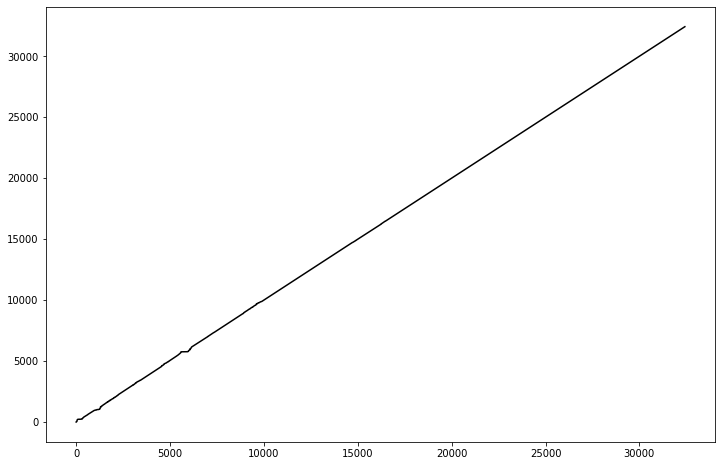
\includegraphics[width=0.5\textwidth]{figuras/x0319_warp_path_gt.png}}
  \hfill
  \subfloat[Espectro telúrico de X0319 reconstruído a partir do caminho do DTW]{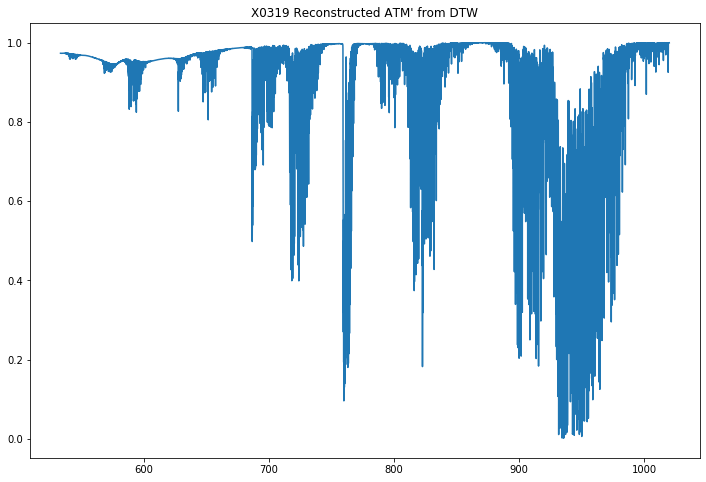
\includegraphics[width=0.5\textwidth]{figuras/x0319_v_n_e_tra_dtw.png}}
  \caption{Caminho do DTW e espectro telúrico reconstruído de X0319}
  \label{fig:x0319-dtw-telluric}
\end{figure}

\begin{figure}[htb]
  \centering
  \subfloat[Caminho do DTW entre espectros telúricos de X0386]{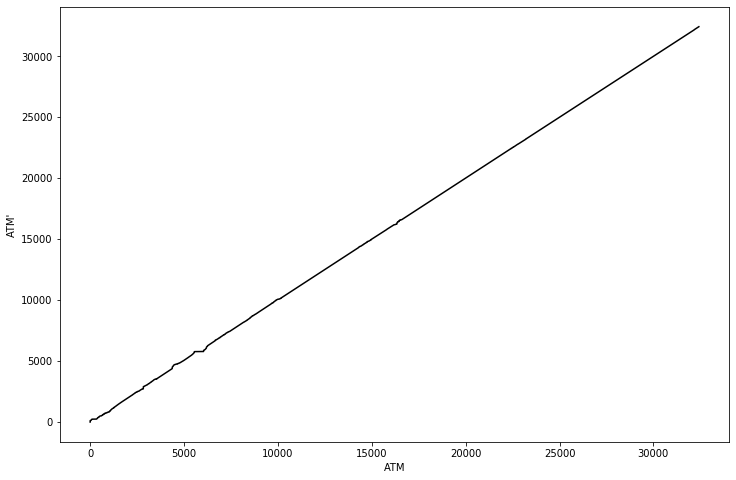
\includegraphics[width=0.5\textwidth]{figuras/x0386_warp_path_gt.png}}
  \hfill
  \subfloat[Espectro telúrico de X0319 reconstruído a partir do caminho do DTW]{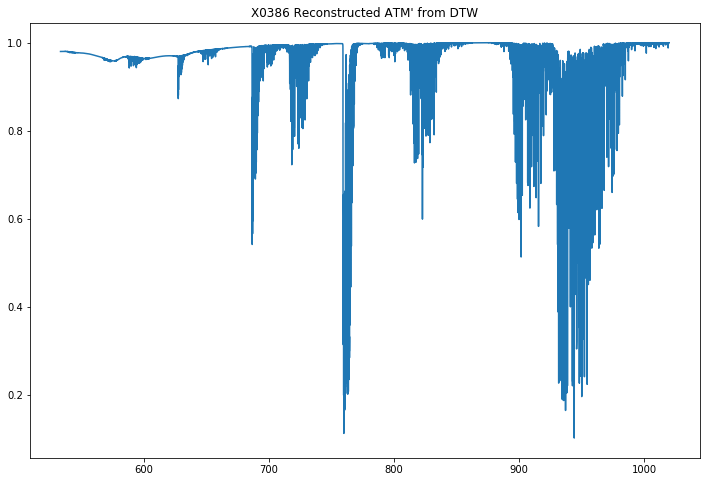
\includegraphics[width=0.5\textwidth]{figuras/x0386_v_n_e_tra_dtw.png}}
  \caption{Caminho do DTW e espectro telúrico reconstruído de X0319}
  \label{fig:x0386-dtw-telluric}
\end{figure}

% resultados dtw
As figuras~\ref{fig:x0319-dtw-telluric} e~\ref{fig:x0386-dtw-telluric} mostram os caminhos resultantes da aplicação do DTW nos espectros telúricos do \texttt{Molecfit} e nos espectros telúricos \textit{ground-truth} de X0319 e X0386. Diferentemente dos caminhos resultantes do DTW quando aplicados no sinal estelar e telúrico, neste caso quase não existem distorções e o caminho se aproxima do caso ideal. Os pequenos desvios em relação à diagonal no caminho resultante indicam desalinhamentos no sinal estelar que foram manualmente corrigido pelo grupo de pesquisadores responsável pelo espectro final. 
% metrica de shift
Para melhor compreender as regiões do espectro telúrico mais afetadas por desalinhamentos, foi computada uma função \textit{shift} ao longo do caminho do DTW, tal que, para cada par de índices $(i,j)$ desse caminho, o valor do \textit{shift} é representado por $j - i$. Desta forma é possível ver os desalinhamentos em termos de quantidade de índices de desvio entre os respectivos sinais telúricos.

\begin{figure}[htb]
\centering
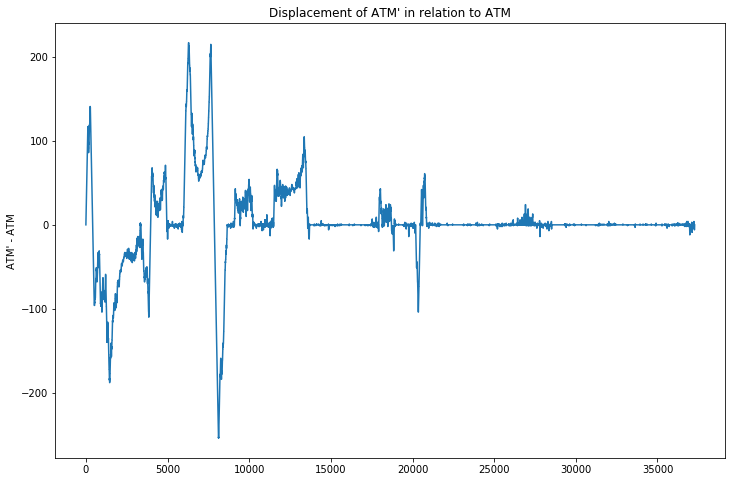
\includegraphics[width=10cm]{figuras/x0386_displacement.png}
\caption{Desalinhamentos em número de elementos entre o modelo do \texttt{Molecfit} e o espectro telúrico realinhado de X0386}
\label{fig:x0386-displacement}
\end{figure}

% resultado do shift
A figura~\ref{fig:x0386-displacement} ilustra a magnitude dos desalinhamentos entre o espectro dado do \texttt{Molecfit} e o espectro telúrico realinhado da estrela X0386. Os maiores desalinhamentos são adiantamentos ou atrasos em 200 elementos dos vetores que representam os espectros, o que representa desalinhamentos em comprimento de onda de aproximadamente 3\,nm. Isto acontece principalmente entre o elemento 5000 e 10000 dos vetores, que é a região de 608\,nm a 683\,nm.

% conclusão do experimento (como melhorar?)
Este resultado ilustra uma aplicação possível do algoritmo DTW em vetores que representam a mesma informação, nesse caso entre dois espectros telúricos antes e depois de um realinhamento realizado por especialistas. Tal aplicação poderia ser de interesse em tarefas de aprendizado automático relacionadas com correção de desalinhamentos instrumentais, por exemplo.

